The completed experiment contains 350 series from 23 source
families, 1050 released score vectors, and 2100 score/width
evaluations. Sequence lengths range from 1,000 to
900,000. The independent final artifact gate passes all
coverage, finite-value, source-hash, internal, crop, and external-comparator checks.
The maximum absolute numerical discrepancy is $3.69\times10^{-13}$.

The median compiled-sparse speedup over the fastest dense baseline is
2.06$\times$, with geometric mean 2.02$\times$.
The 95\% series-cluster bootstrap interval for the geometric mean is
[1.93, 2.12]; resampling whole source families gives
[1.56, 2.48]. These are descriptive uncertainty summaries
for the fixed corpus. Sparse evaluation is faster in 1916 of
2100 cases, while 184 cases are slower or equal.
The full speedup range is 0.27--7.50$\times$.
Figure~\ref{fig:results} retains these slowdowns rather than filtering dense support.

\begin{figure}[t]
\centering
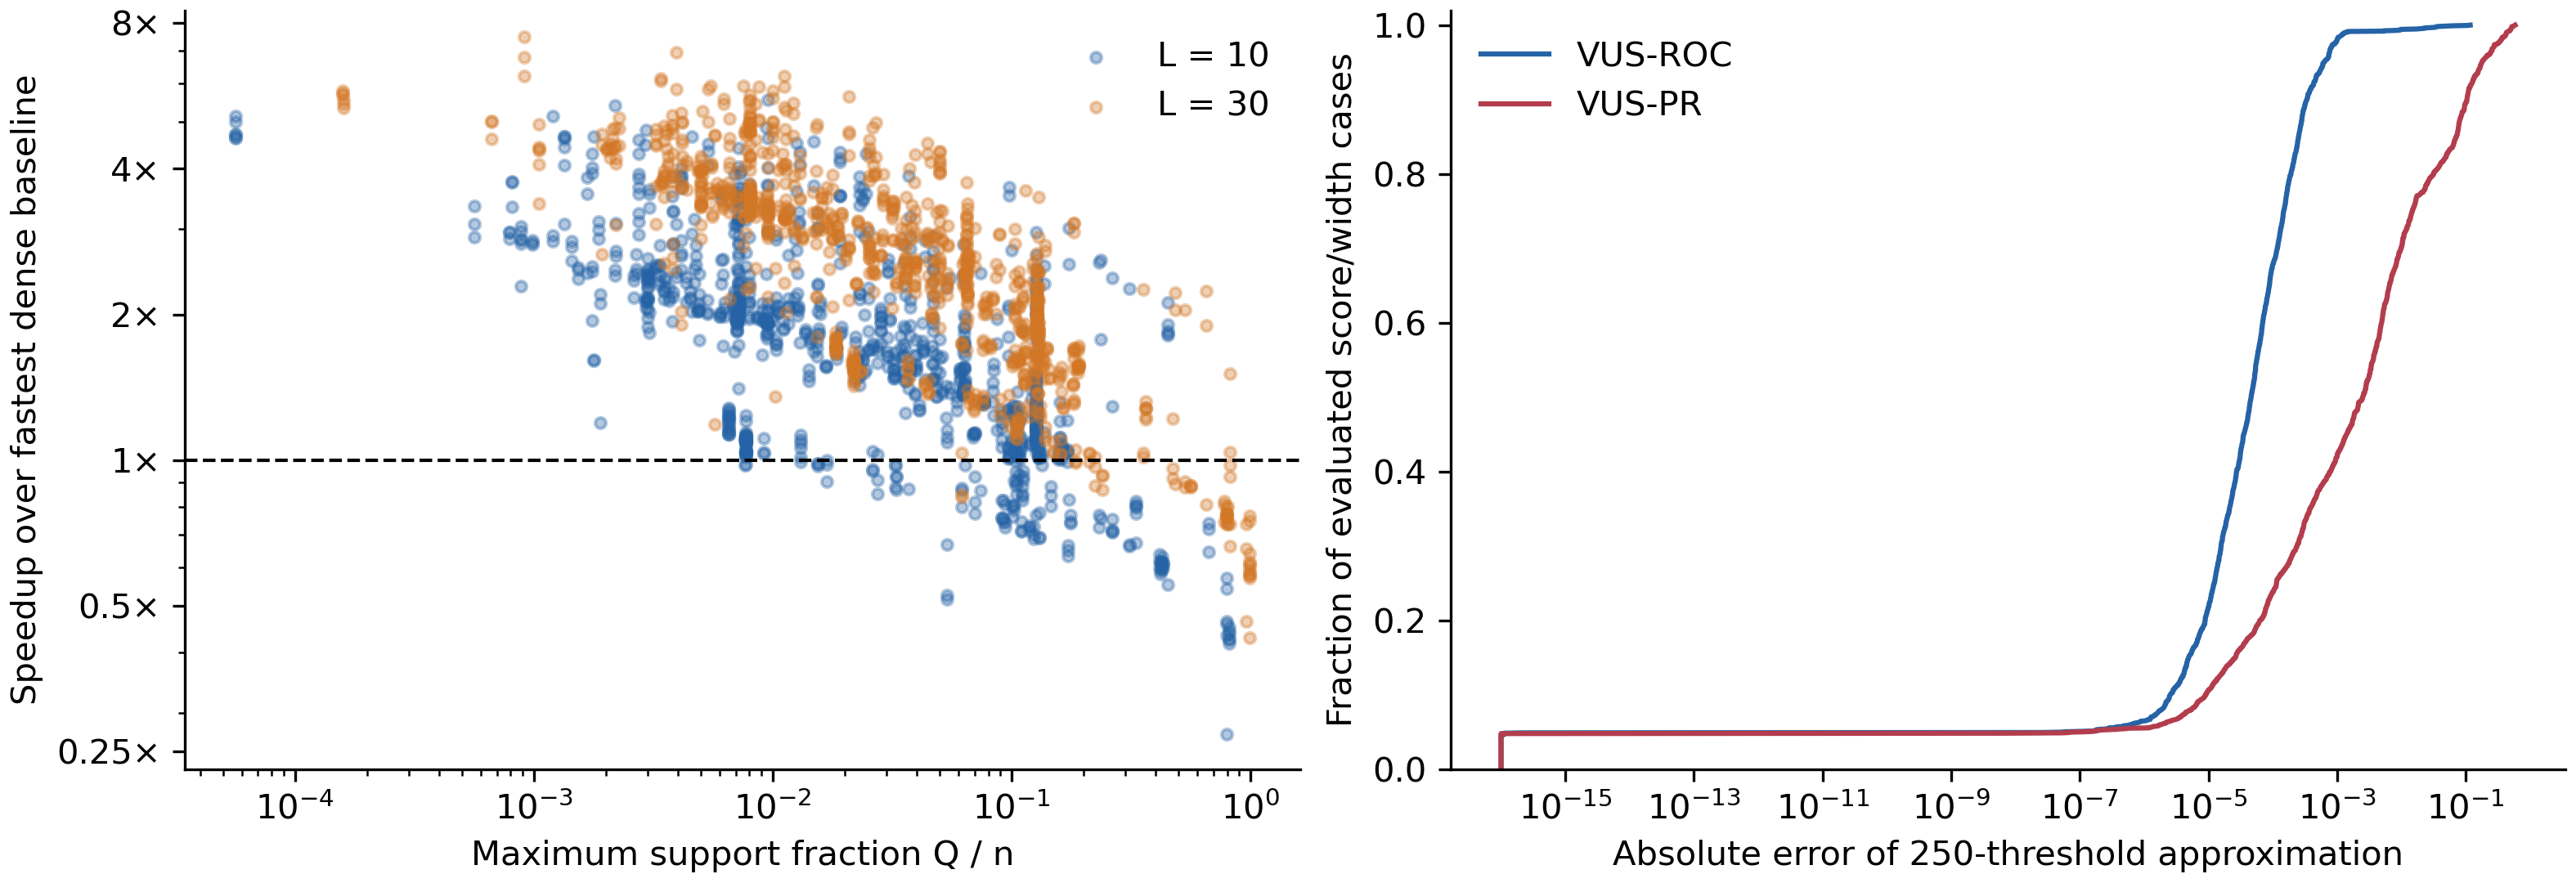
\includegraphics[width=\linewidth]{public-results.png}
\caption{Left: all 2100 paired runtime comparisons, using the fastest of three dense
implementations per input. Right: threshold-sampling error on the same fixed score vectors.
Zero errors are displayed at $10^{-16}$ for the logarithmic axis.}
\label{fig:results}
\end{figure}

\begin{table}[htbp]
\centering
\begin{tabular}{lrrrr}
\toprule
Metric & Median error & 95th percentile & Maximum error & Reversals / pairs \\
\midrule
VUS-ROC & $4.59\times10^{-5}$ & $6.21\times10^{-4}$ & $0.117$ & 5 / 2100 \\
VUS-PR & $2.50\times10^{-3}$ & $0.178$ & $0.583$ & 84 / 2100 \\
\bottomrule
\end{tabular}
\caption{Errors are absolute differences between the same metric at 250 sampled thresholds and all thresholds. Reversals require strict opposite order in both calculations.}
\label{tab:sampling}
\end{table}

For VUS-ROC, strict reversals occur on 2 unique series across 2 families, and the unique top model changes in 2 of 700 series/width cases. Exact and sampled comparisons contain 96 and 95 ties, respectively.

For VUS-PR, strict reversals occur on 55 unique series across 13 families, and the unique top model changes in 50 of 700 series/width cases. Exact and sampled comparisons contain 96 and 95 ties, respectively.

The largest observed PR discrepancy occurs on the 195,000-point UCR HumanActivity series with Time-MoE scores and $L=30$: exact VUS-PR is 0.666890, versus 0.084159 at 250 thresholds. The scores are unchanged between calculations.

On the bounded 12-series NAB external comparison, the median speed ratios relative to compiled sparse evaluation are 53.86$\times$ for full-threshold dtaianomaly, 8.92$\times$ for 250-threshold dtaianomaly, and 149.29$\times$ for official 250-threshold evaluation. The latter two compare exact computation with a coarser approximation. These results do not establish the same advantage on other families or against the unavailable accelerated VUS implementation.

In the frozen fixed-support scaling experiment ($Q=102$, $L=30$), the one-million-point case takes 0.0626 seconds for compiled sparse evaluation, an 8.92$\times$ speedup over the fastest dense implementation, with five randomized-order repetitions.

\subsection{Mechanism and the density/width tradeoff}
On the 112-case synthetic grid, replacing full-score sorting with
support-score counting gives a geometric-mean end-to-end speedup of
1.11$\times$ with the same integration kernel,
range 0.94--1.80$\times$.
The adapter deliberately holds support grouping and all other preparation
fixed, isolating the score-counting choice. Relative to the fastest dense
implementation, the complete sparse method has geometric-mean speedup
1.37$\times$, range
0.26--7.53$\times$.
There are 69 cases with at least a 1.1$\times$
speed ratio and 34 with ratio at most $1/1.1$.
The remaining cases lie between those thresholds. Thus the count-preprocessing
improvement is modest on this grid; sparse event integration supplies the
larger opportunity as support shrinks and the width range grows.

\begin{figure}[t]
\centering
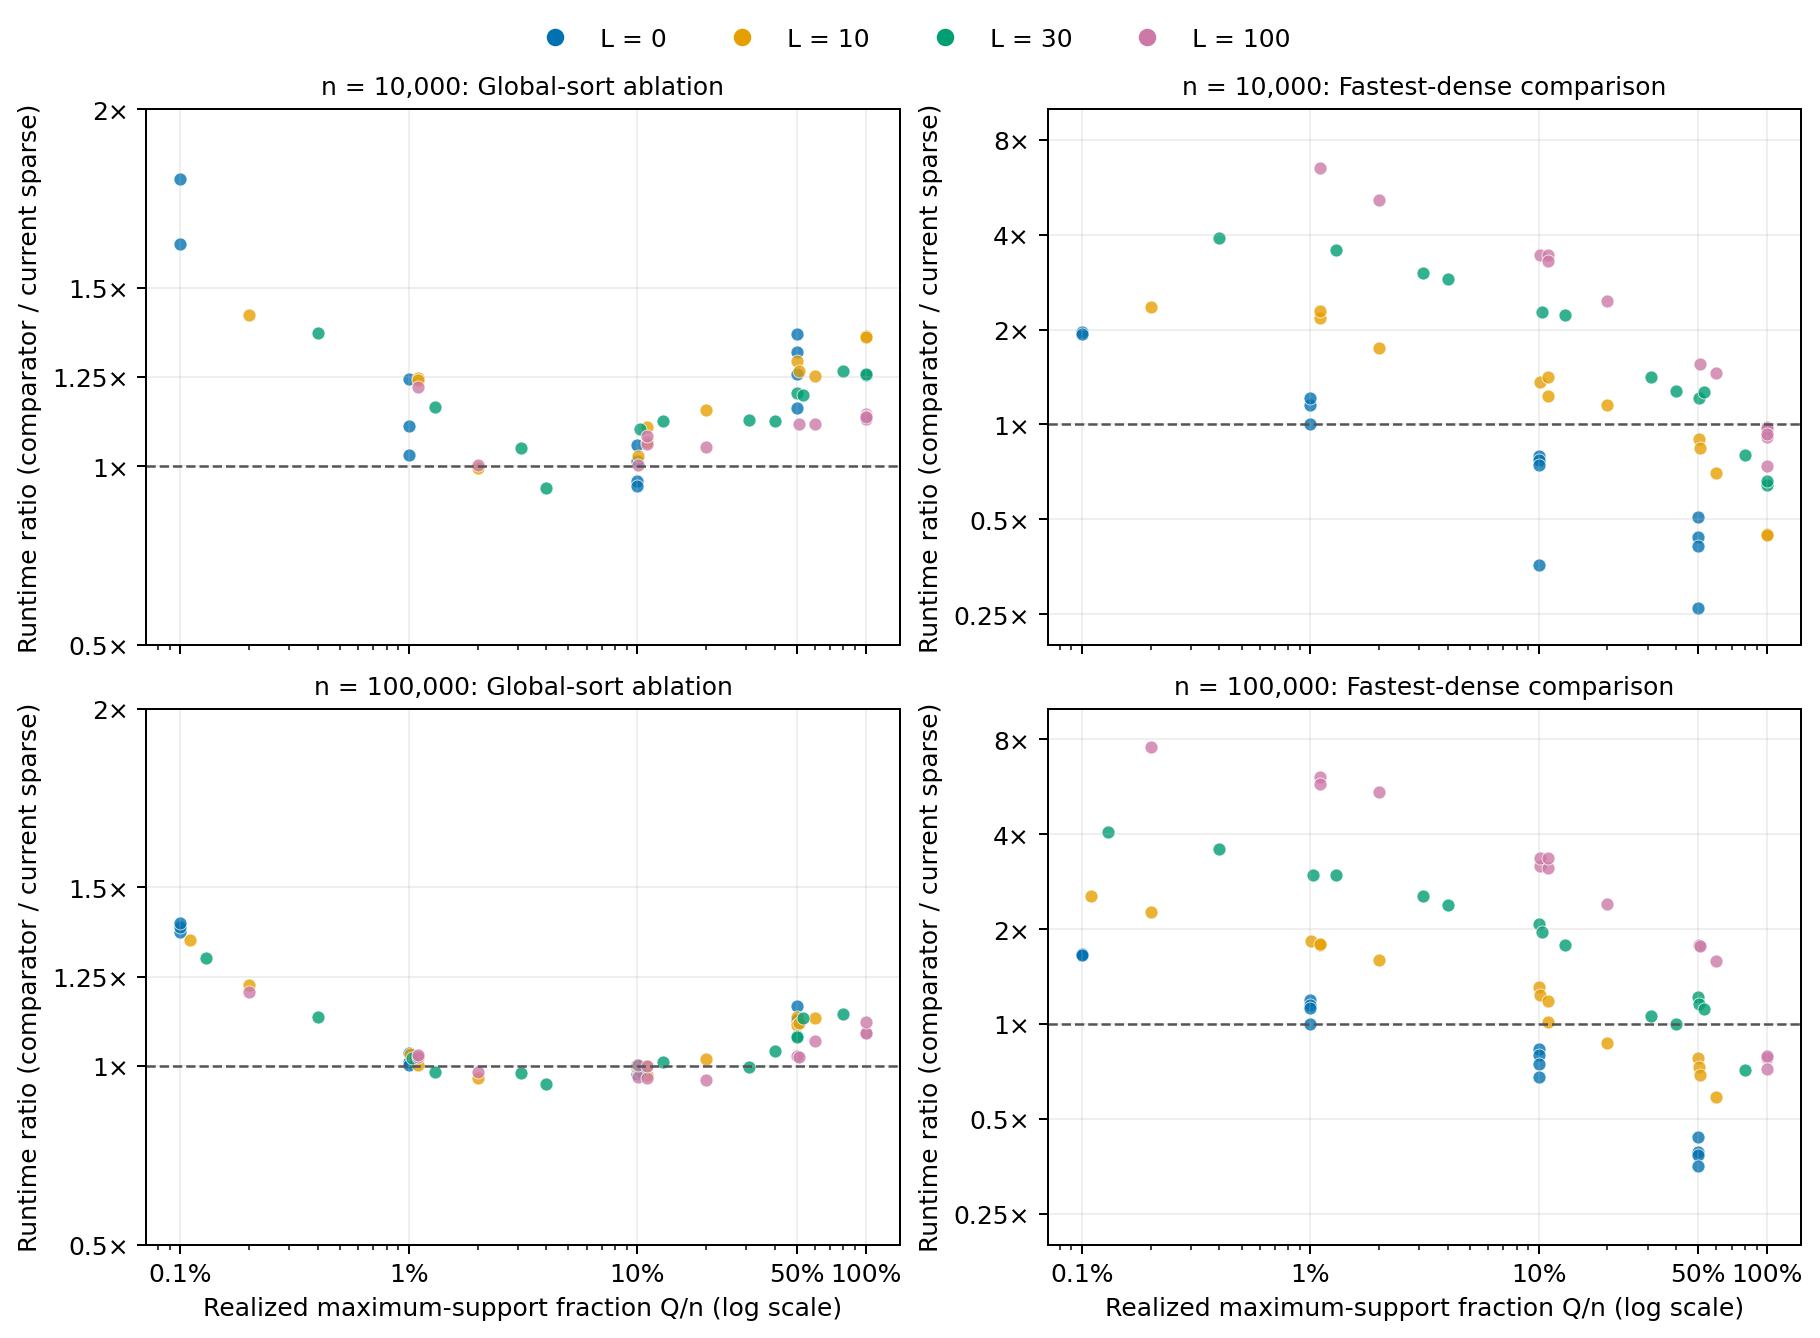
\includegraphics[width=\linewidth]{figures/mechanism.readable.png}
\caption{Mechanism ablation: each point is one predeclared synthetic cell,
using medians of three randomized repetitions. Support fraction $Q/n$ is
measured after expansion. The dense comparator is the fastest of three dense
implementations. The full-sort variant keeps support grouping and the compiled
sparse integration kernel fixed.}
\label{fig:mechanism}
\end{figure}

\subsection{Published implementation across source families}
The post-review supplement selects the shortest and median-length series
within each family, deduplicating coincident choices. It contains
42 full-length series from all 23
families, uses Chronos-Bolt base scores and $L=30$, and preserves all vectors.
Methods run in a seeded random order, with three repetitions per method.
Each call has a ten-second post-warmup time limit; late or unfinished calls
are recorded as right-censored. Compilation and subprocess startup are
excluded. Table~\ref{tab:external} reports speed ratios only for completed
pairs, whose subset differs across threshold modes. No numerical speed ratio
is imputed for a censored result.

\begin{table}[htbp]
\centering
\begin{tabular}{lrrrr}
\toprule
dtaianomaly mode & Completed & Censored & Families represented & Median ratio \\
\midrule
250 thresholds & 42 & 0 & 23 & 8.17$\times$ \\
All thresholds & 35 & 7 & 19 & 143.85$\times$ \\
\bottomrule
\end{tabular}
\caption{Actual pinned dtaianomaly code on 42 source-stratified
full-length inputs. Ratios divide the published baseline's median time by
compiled sparse exact evaluation. The 250-threshold row compares an
approximation with exact computation. Completion-conditioned medians are
not full-corpus runtime estimates. Family counts require at least one completed
pair within the family.}
\label{tab:external}
\end{table}

The maximum absolute discrepancy for returned outputs, compared with the
corresponding exact or 250-threshold main result, is
$9.55\times10^{-15}$. All selection, timeout, environment,
and per-call receipts are retained.
